\documentclass[10pt]{beamer}

\usetheme[progressbar=frametitle]{metropolis}
\usepackage{appendixnumberbeamer}

\usepackage{booktabs}
\usepackage[scale=2]{ccicons}

\usepackage{pgfplots}
\usepgfplotslibrary{dateplot}

\usepackage{xspace}
\newcommand{\themename}{\textbf{\textsc{metropolis}}\xspace}

\usepackage{caption}
%\usepackage{gensymb}
\usepackage{ulem}
\usepackage{subcaption}
\usepackage[french]{babel}
\usepackage{csquotes}
\usepackage[backend=biber,style=authoryear,citestyle=authoryear]{biblatex}
\usepackage{tikz}
\usetikzlibrary{positioning}

\DeclareCaptionLabelFormat{underlcap}{\uline{#1 #2}}
\DeclareCaptionLabelSeparator{underlcap}{~}
\DeclareCaptionTextFormat{underlcap}{\expandafter\uline\expandafter{\expandafter#1}}

\captionsetup[figure]{%
   labelformat=underlcap,labelseparator=underlcap,textformat=underlcap}
   
\newcommand\Wider[2][3em]{%
\makebox[\linewidth][c]{%
  \begin{minipage}{\dimexpr\textwidth+#1\relax}
  \raggedright#2
  \end{minipage}%
  }%
}

\makeatletter
\setlength{\metropolis@progressinheadfoot@linewidth}{1.7pt}
\setlength{\metropolis@titleseparator@linewidth}{1.7pt}
\setlength{\metropolis@progressonsectionpage@linewidth}{1.7pt}

\definecolor{alizarin}{rgb}{0.1, 0.26, 0.82}
\definecolor{bazaar}{rgb}{0.63, 0.63, 0.8}

\setbeamercolor{progress bar}{fg=alizarin,bg=bazaar}

\AtBeginSection[]{
  \begin{frame}
  \vfill
  \centering
  \begin{beamercolorbox}[sep=8pt,center,shadow=true,rounded=true]{title}
    \usebeamerfont{title}\insertsectionhead\par%
  \end{beamercolorbox}
  \vfill
  \end{frame}
}

\definecolor{felixlightblue}{rgb}{0.85, 0.85, 0.99}
% \metroset{block=fill}
\setbeamercolor{block body}{bg=felixlightblue}

\addbibresource{/Applications/ZoteroBibs/Library.bib}

\title{Impact de l'organisation de la convection profonde sur l'humidité troposphérique}
\subtitle{Félix Langot}
\date{\today}
\author{Supervisé par Dr. C. Risi \newline \textit{LMD - UVSQ/Paris-Saclay}}
\institute{\vspace{0.7cm}
\includegraphics[width=4.5cm]{Figures/LMDSorbonne.png}\hfill\includegraphics[width=3.3cm]{/Users/felixlangot/Pictures/Icons/logo-uvsq-2020-actu.png}}

\begin{document}
{\usebackgroundtemplate{\tikz\node[opacity=0.2, anchor=center]{\includegraphics[width=21cm]{/Users/felixlangot/Google Drive (felixlangot@gmail.com)/UVSQ/Gestion de Projet/Poster/wallpaper2you_568686.jpg}};}
% {\usebackgroundtemplate{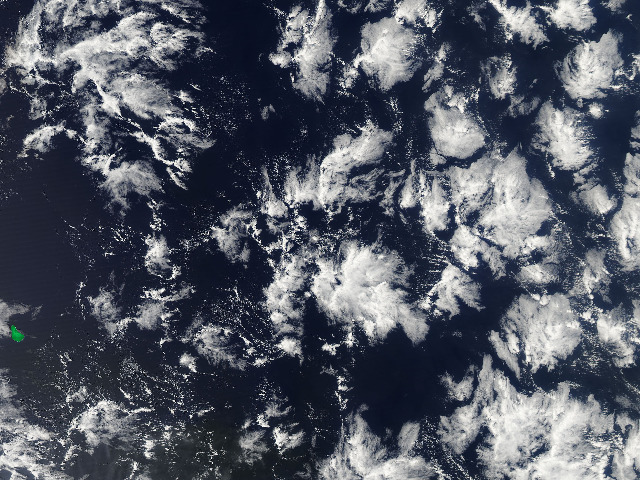
\includegraphics{Figures/Flowers.jpeg}}
\begin{frame}[plain,noframenumbering]
  \maketitle
\end{frame}
}

\section*{Introduction}

\begin{frame}{\secname}
\Wider{
    \vspace{0.2cm}
    \begin{itemize}
        \item Convection profonde = grands nuages, associés aux orages
        \item Différents types d'organisation de la convection profonde
        \item Organisation plus forte encouragée par réchauffement de SST
        \item + d'organisation $\rightarrow$ assèchement de la troposphère
    \end{itemize}
    $\rightarrow$ Potentielle rétroaction climatique \\
    \vspace{4cm}
    \begin{tikzpicture}[overlay, remember picture]
        \node[above =1.6cm of current page.south]
        {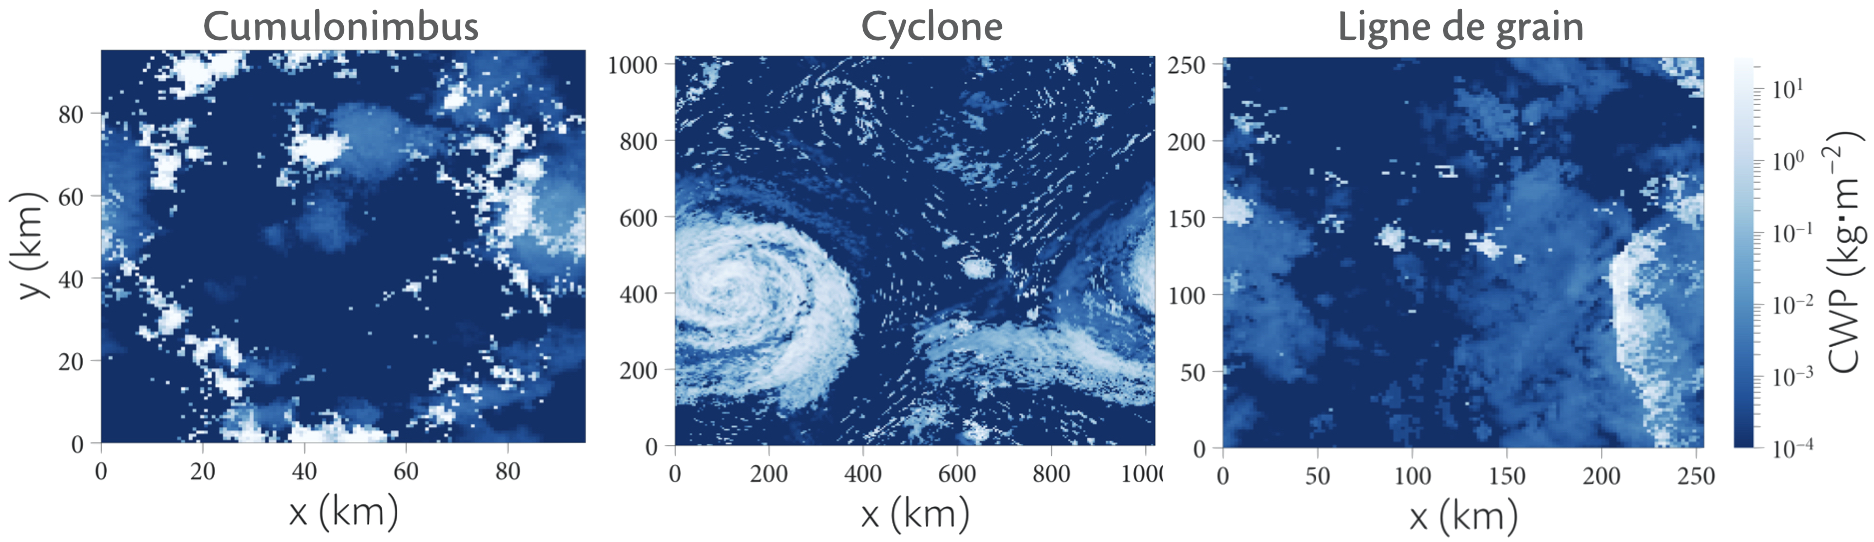
\includegraphics[width=12cm]{Figures/VisAssemble2.png}};
    \end{tikzpicture}
    \textbf{But du stage:} développer un modèle théorique simple pour comprendre l'effet de l'organisation de la convection sur l'humidité de la troposphère 
}
\end{frame}


% \begin{frame}{\secname}

%     \begin{itemize}
%         \setlength{\itemsep}{7pt}
%         \item \textbf{But du stage:} développer un modèle théorique simple pour quantifier l'effet de l'organisation de la convection sur l'humidité de la troposphère 
%         \item Utilisation de simulations CRM $\rightarrow$ vérifier les hypothèses du modèle simple + évaluer son réalisme. 
%         \item Différentes distributions de l'humidité relative (RH) dans la troposphère, dues à: \\
%         $\rightarrow$ l'agrégation de la convection: fait baisser la RH  \autocite{Tobin2012} \\
%         $\rightarrow$ l'ascendance: humidifie la troposphère \autocite{brethertonRelationshipsWaterVapor2004} \\
%     \end{itemize}

% \end{frame}

\begin{frame}{\secname}
\Wider{
\textbf{Simulation en équilibre radiatif-convectif (RCE) avec le Cloud-Resolving  Model  (CRM) SAM:}
\begin{figure}[hbtp]
    \centering
    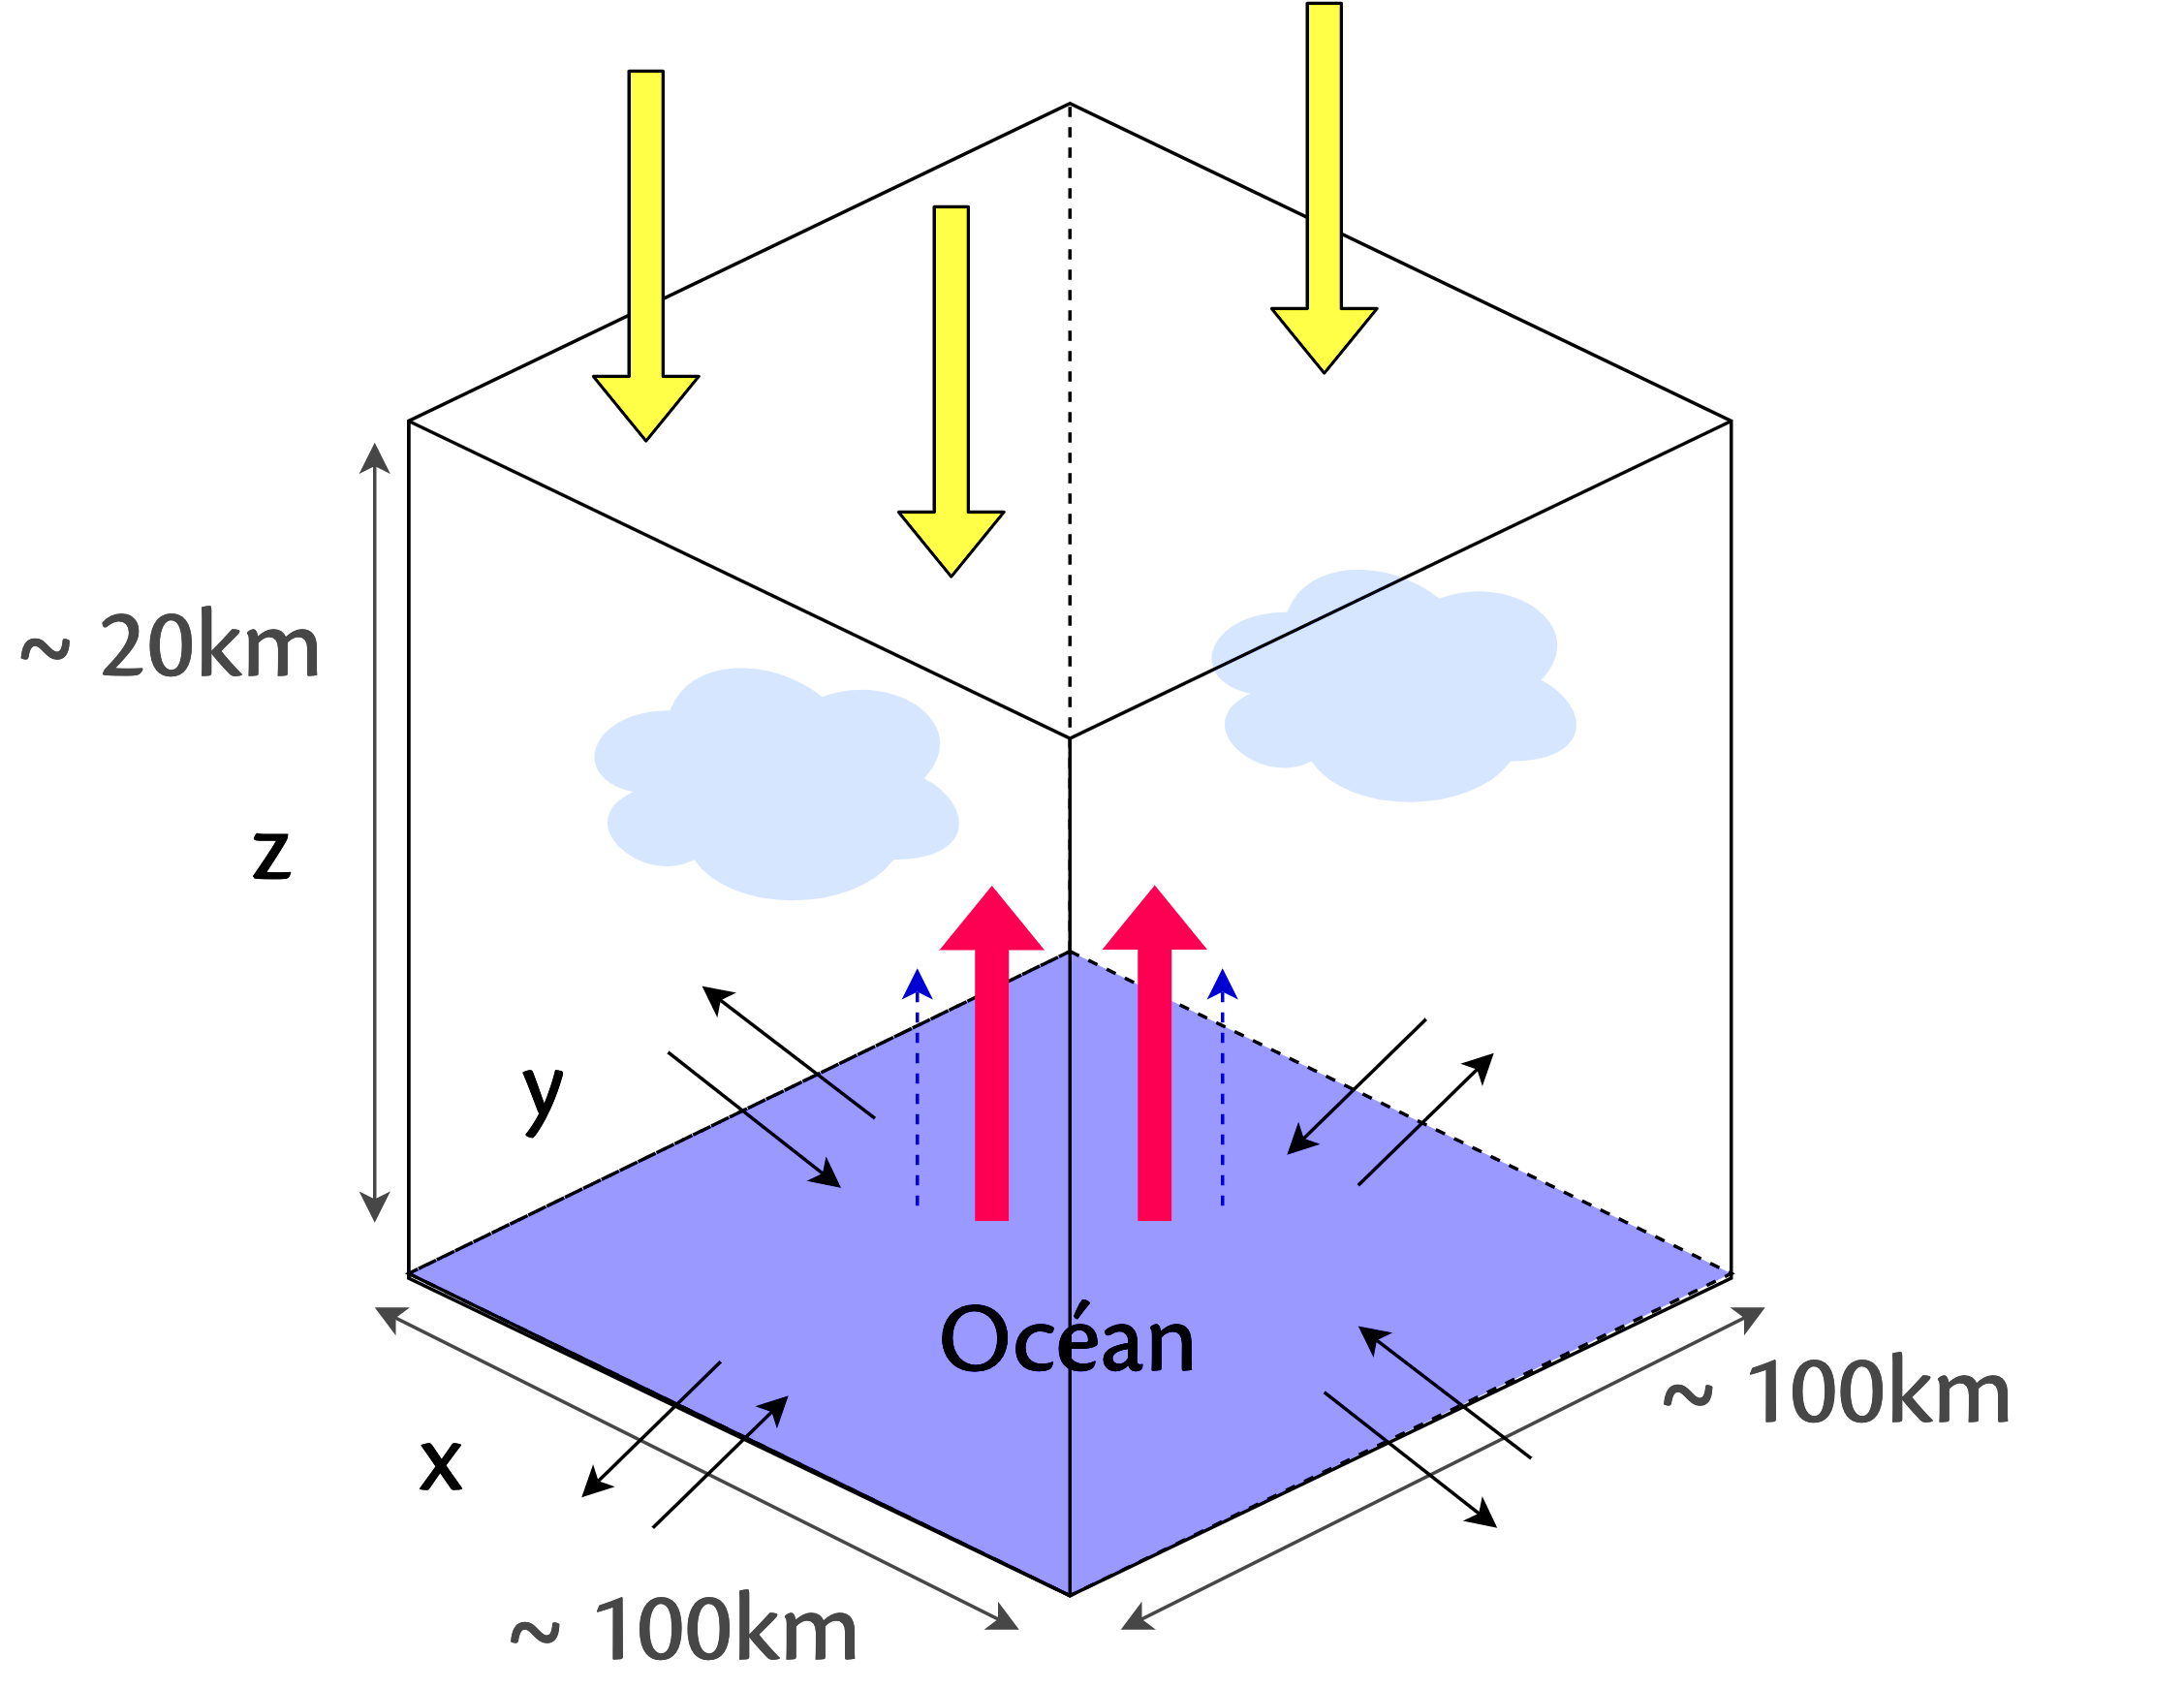
\includegraphics[width=8cm]{Figures/CRM.png}  
\end{figure}
}
\end{frame}

\begin{frame}{\secname}
\Wider{
 \textbf{Simulation en équilibre radiatif-convectif (RCE) avec le Cloud-Resolving  Model  (CRM) SAM:}
 \vspace{-0.5cm}
\begin{figure}[hbtp]
    \centering
    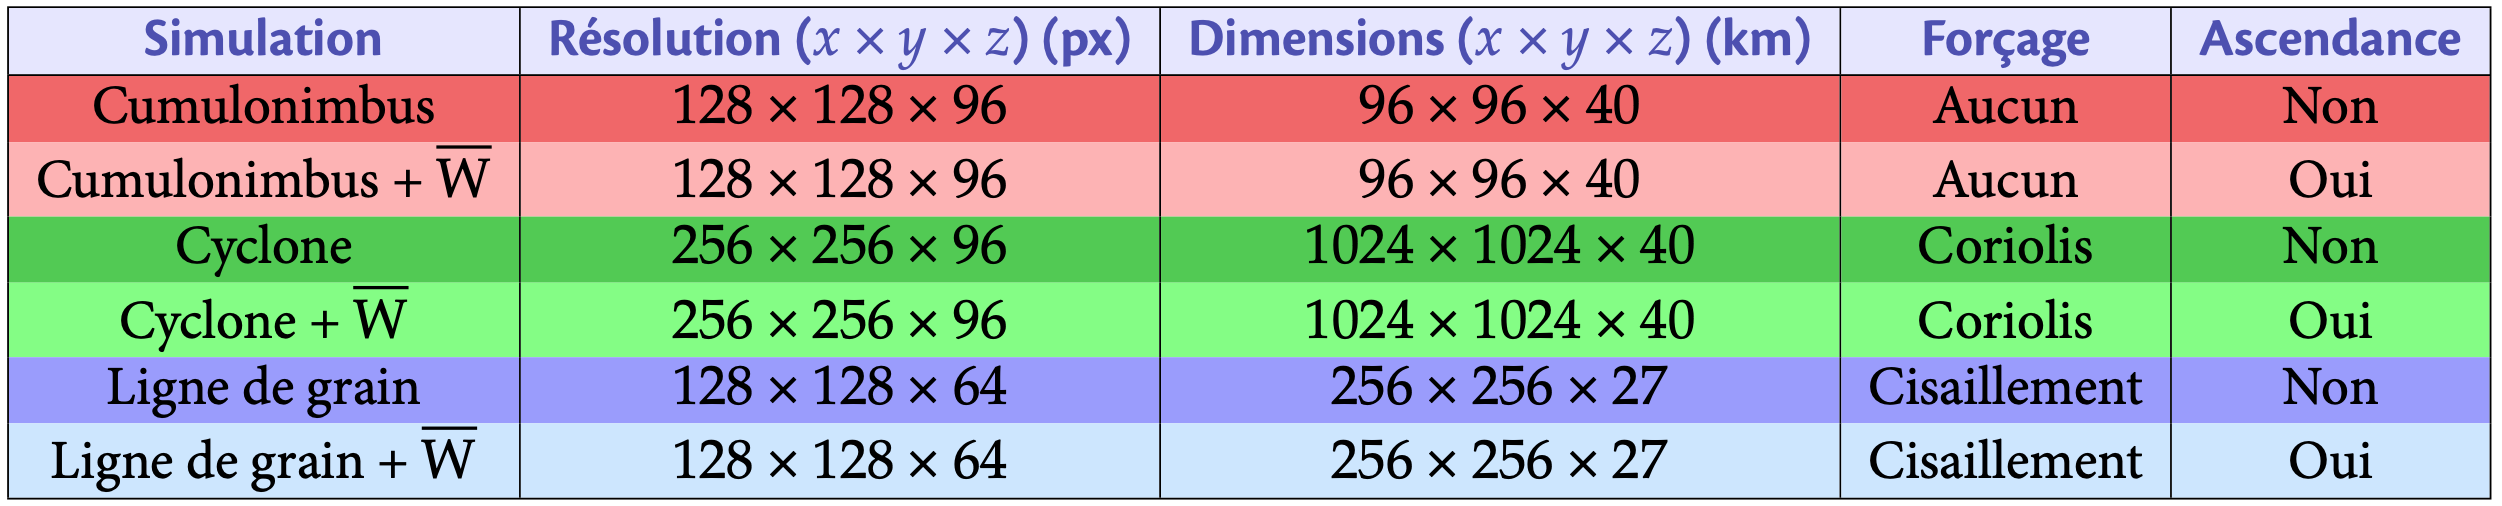
\includegraphics[width=12cm]{Figures/TableExp.png}  
\end{figure}
\begin{columns}
    \column{0.4\textwidth}
    $$RH_{a} = \left. \ \frac{q_{v}}{q_{sat}} \right|_{z_{parcel} = 5km}$$ 
    \column{0.6\textwidth}
    \includegraphics[width=6.5cm]{../Codes/Figs/Rhmeancomps.png}
\end{columns}
}
\end{frame}

\section*{Comment prédire la \textit{RH} troposphérique?}
\begin{frame}{\secname}
\Wider{
\begin{itemize}
    \item \textbf{Hypothèse 1:} Les changements d'humidité sont liés aux effets dynamiques de l'organisation de la convection  
    \item \textbf{Hypothèse 2:} Les effets microphysiques liés à l'évaporation de la pluie ou au détrainement de la convection gouvernent l'humidité
\end{itemize}
}
\vspace{-1cm}
\pause
    \begin{columns}
        \column{0.55\textwidth}
        \begin{itemize}
            \item Modèle d'advection- condensation (AC) \autocite{sherwoodMaintenanceFreeTroposphericTropical1996,pierrehumbertRelativeHumidityAtmosphere2007}
            \item Prédiction de l'humidité: $$RH_{p} = \frac{q_{sat}(z_{clouds})}{q_{sat}(z_{parcel})}$$
            \item Organisation $\rightarrow$ probabilité de saturation
        \end{itemize}
        \column{0.6\textwidth}
        \begin{figure}[hbtp]
            \centering
            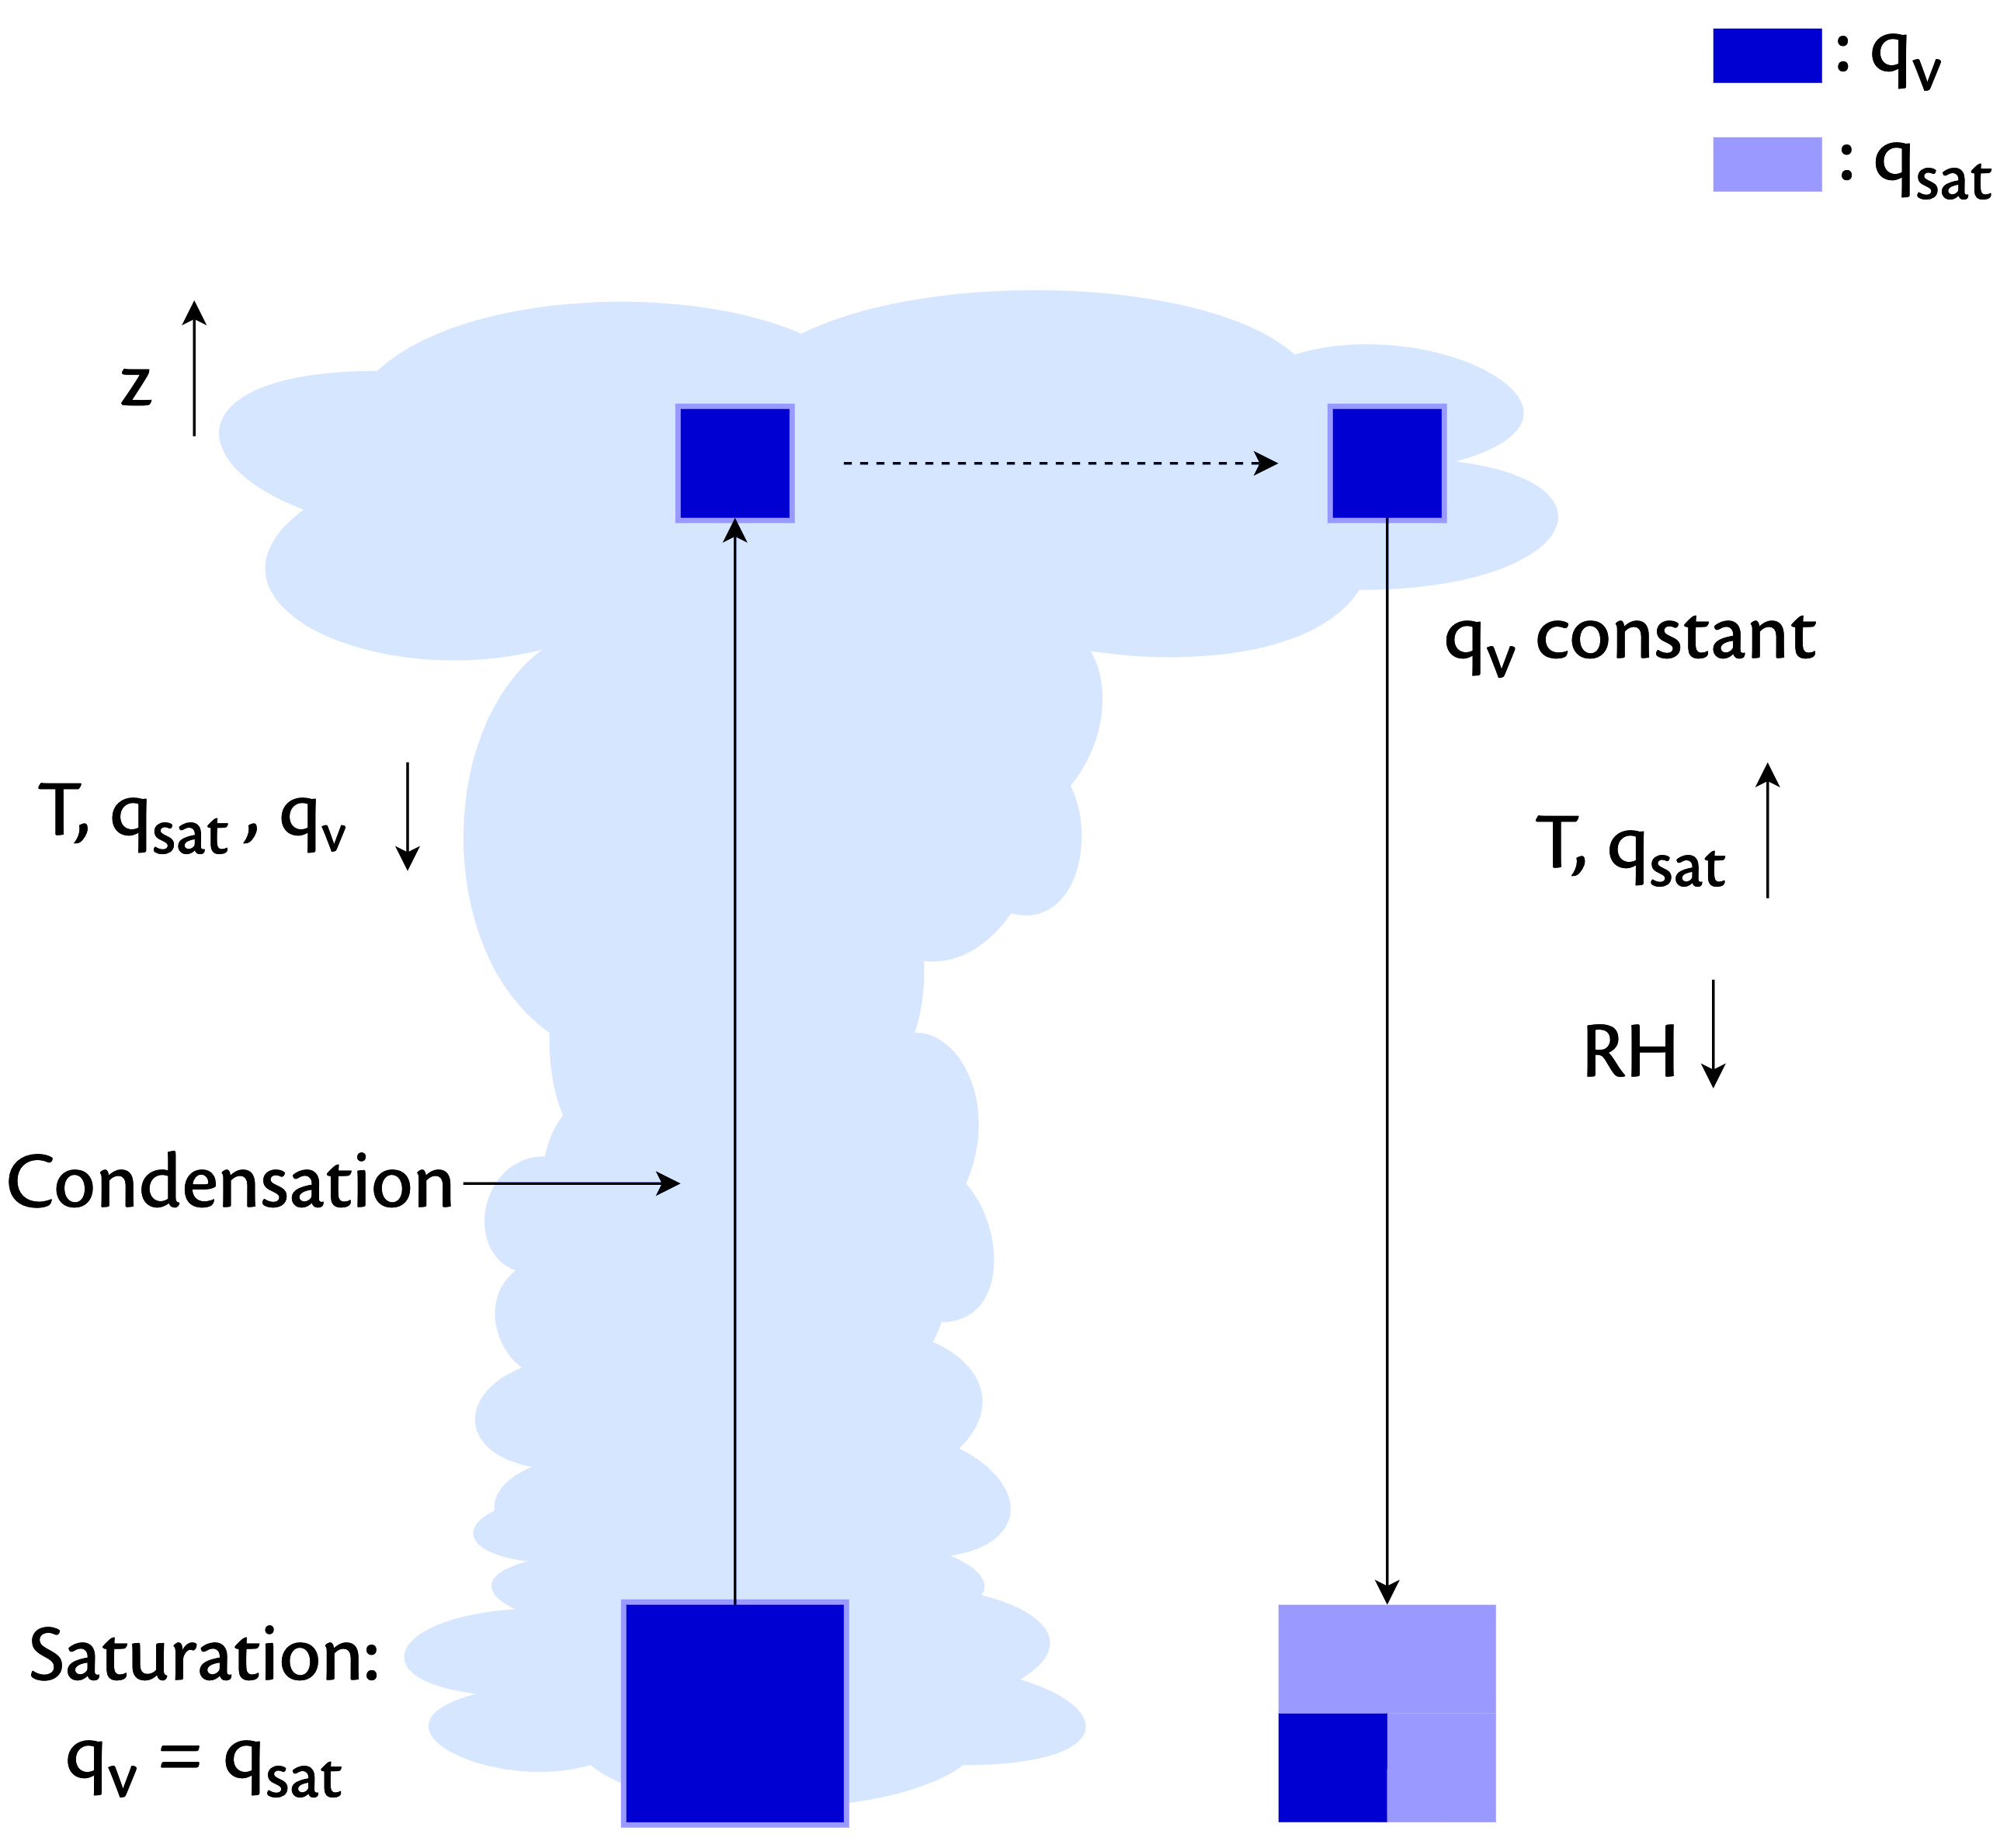
\includegraphics[width=6.6cm]{Figures/advec-condens.png}
        \end{figure}
    \end{columns}

\end{frame}

\section*{Altitude de dernière saturation - Approche statique}
\begin{frame}{\secname}
\Wider{
    \begin{itemize}
        \setlength{\itemsep}{4pt}
        \item \textbf{Approche statique:} L'altitude de dernière saturation d'une parcelle troposphérique correspond à l'altitude du nuage le plus proche au-dessus de la parcelle.
        \item SAM: $q_c + q_i > 10^{-6}$ alors le point de grille est dans un nuage \autocite{thayer-calderNumericalInvestigationBoundary2015}
    \end{itemize}
}
\begin{figure}[hbtp]
    \centering
    \includegraphics[width=10cm]{../Codes/Figs/lastsaturationlight.png}
\end{figure}
\end{frame}

\begin{frame}{\secname}
    Altitude du nuage le plus proche de chaque point de grille à chaque pas de temps des simulations:
    \begin{figure}[hbtp]
        \centering
        \includegraphics[width=10cm]{../Codes/Figs/3Dclouds.png}
    \end{figure}
\end{frame}

\begin{frame}{\secname}
\Wider{
\begin{figure}[hbtp]
    \centering
    \includegraphics[width=7cm]{../Codes/Figs/meanRHpovsRHa.png} \hfill
    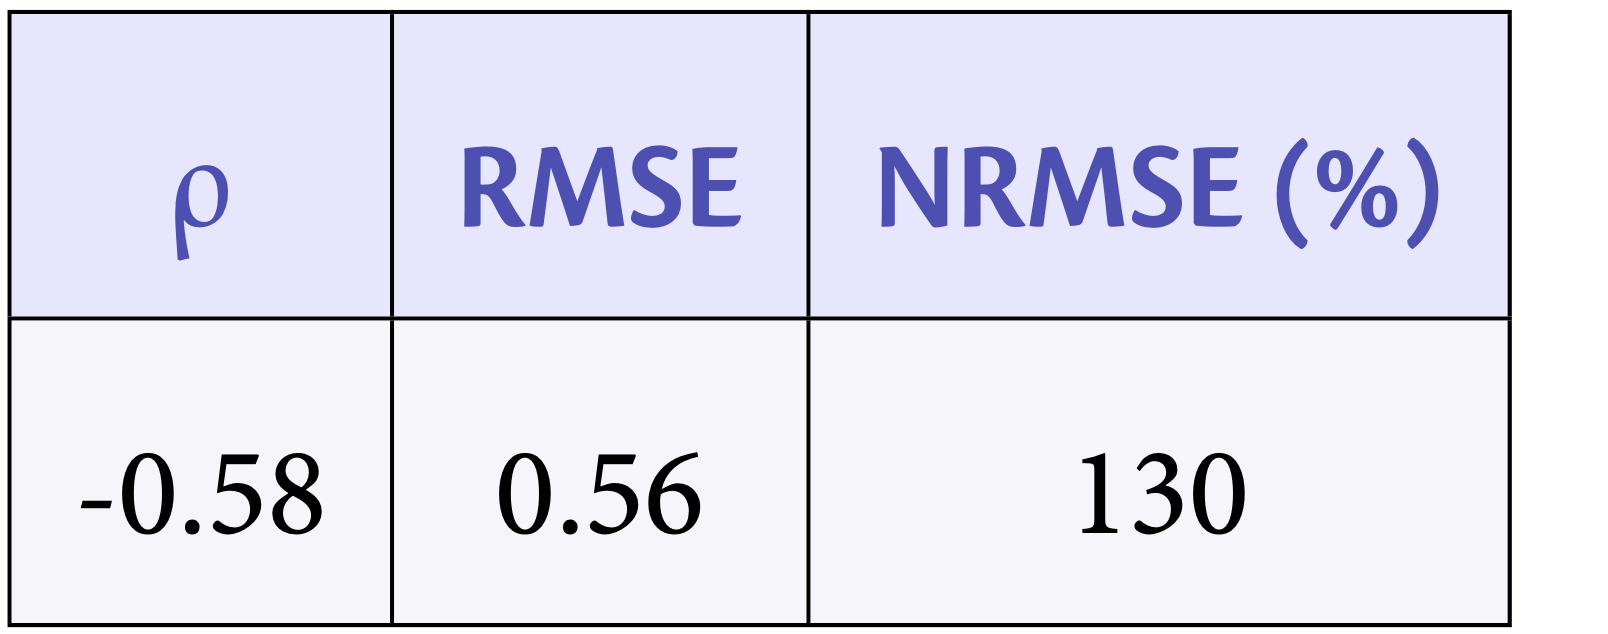
\includegraphics[width=4.5cm]{Figures/Table1.png}
\end{figure}
\vspace{0.2cm}
$\rightarrow$ La $RH$ ne peut pas être prédite par un modèle statique \\ 
$\rightarrow$ Intermittence des nuages + mouvement de la parcelle importants.
}
\end{frame}

\section*{Altitude de dernière saturation - Approche dynamique}

\begin{frame}{\secname}
\Wider{
\textbf{Approche dynamique:} On considère le mouvement vertical d'une parcelle au-dessus de la troposphère.
\vspace{-0.5cm}
\begin{block}{\vspace*{-2.5ex}}
$\rightarrow$ L'altitude de dernière saturation $z_{clouds}$ d'une parcelle à $z_{parcel} =$ 5km au pas de temps $t_N$ est l'altitude à laquelle elle a rencontré un nuage pour la dernière fois le long de sa trajectoire à $t_{N-i}$. 
\end{block}
\begin{figure}[hbtp]
    \centering
    \includegraphics[width=10cm]{../Codes/Figs/lastsaturationsubsidencelight.png}
\end{figure}
}
\end{frame}

\begin{frame}{\secname}
    \begin{itemize}
        \item SAM $\rightarrow w(t,x,y,z) \rightarrow w_{env}(z)$     
        \item Simulations avec ascendance: $w_{tot} = w_{env} + w_{LS}$, où $w_{LS}$ est l'ascendance imposée.
    \end{itemize} 
    \begin{figure}[hbtp]
        \centering
        \includegraphics[width=7cm]{../Codes/Figs/wtotz.png}
    \end{figure}
\end{frame}

\begin{frame}{\secname}
    \begin{itemize}
        \item Pas de temps simulation = 30min
        \item On trace la trajectoire de la parcelle, gouvernée par $w_{tot}$.
    \end{itemize}
    \begin{figure}[hbtp]
        \centering
        \includegraphics[width=8.5cm]{../Codes/Figs2/ztraj.png}
    \end{figure}
\end{frame}

\begin{frame}{\secname}
    En utilisant les mêmes conditions pour détecter les nuages, on obtient les altitudes de dernières saturations suivantes:
    \begin{figure}[hbtp]
        \centering
        \includegraphics[width=10cm]{../Codes/Figs2/zclouds_traj.png}
    \end{figure}
\end{frame}

\section*{Résultats}

\begin{frame}{\secname}
\Wider{
\begin{figure}[hbtp]
    \centering
    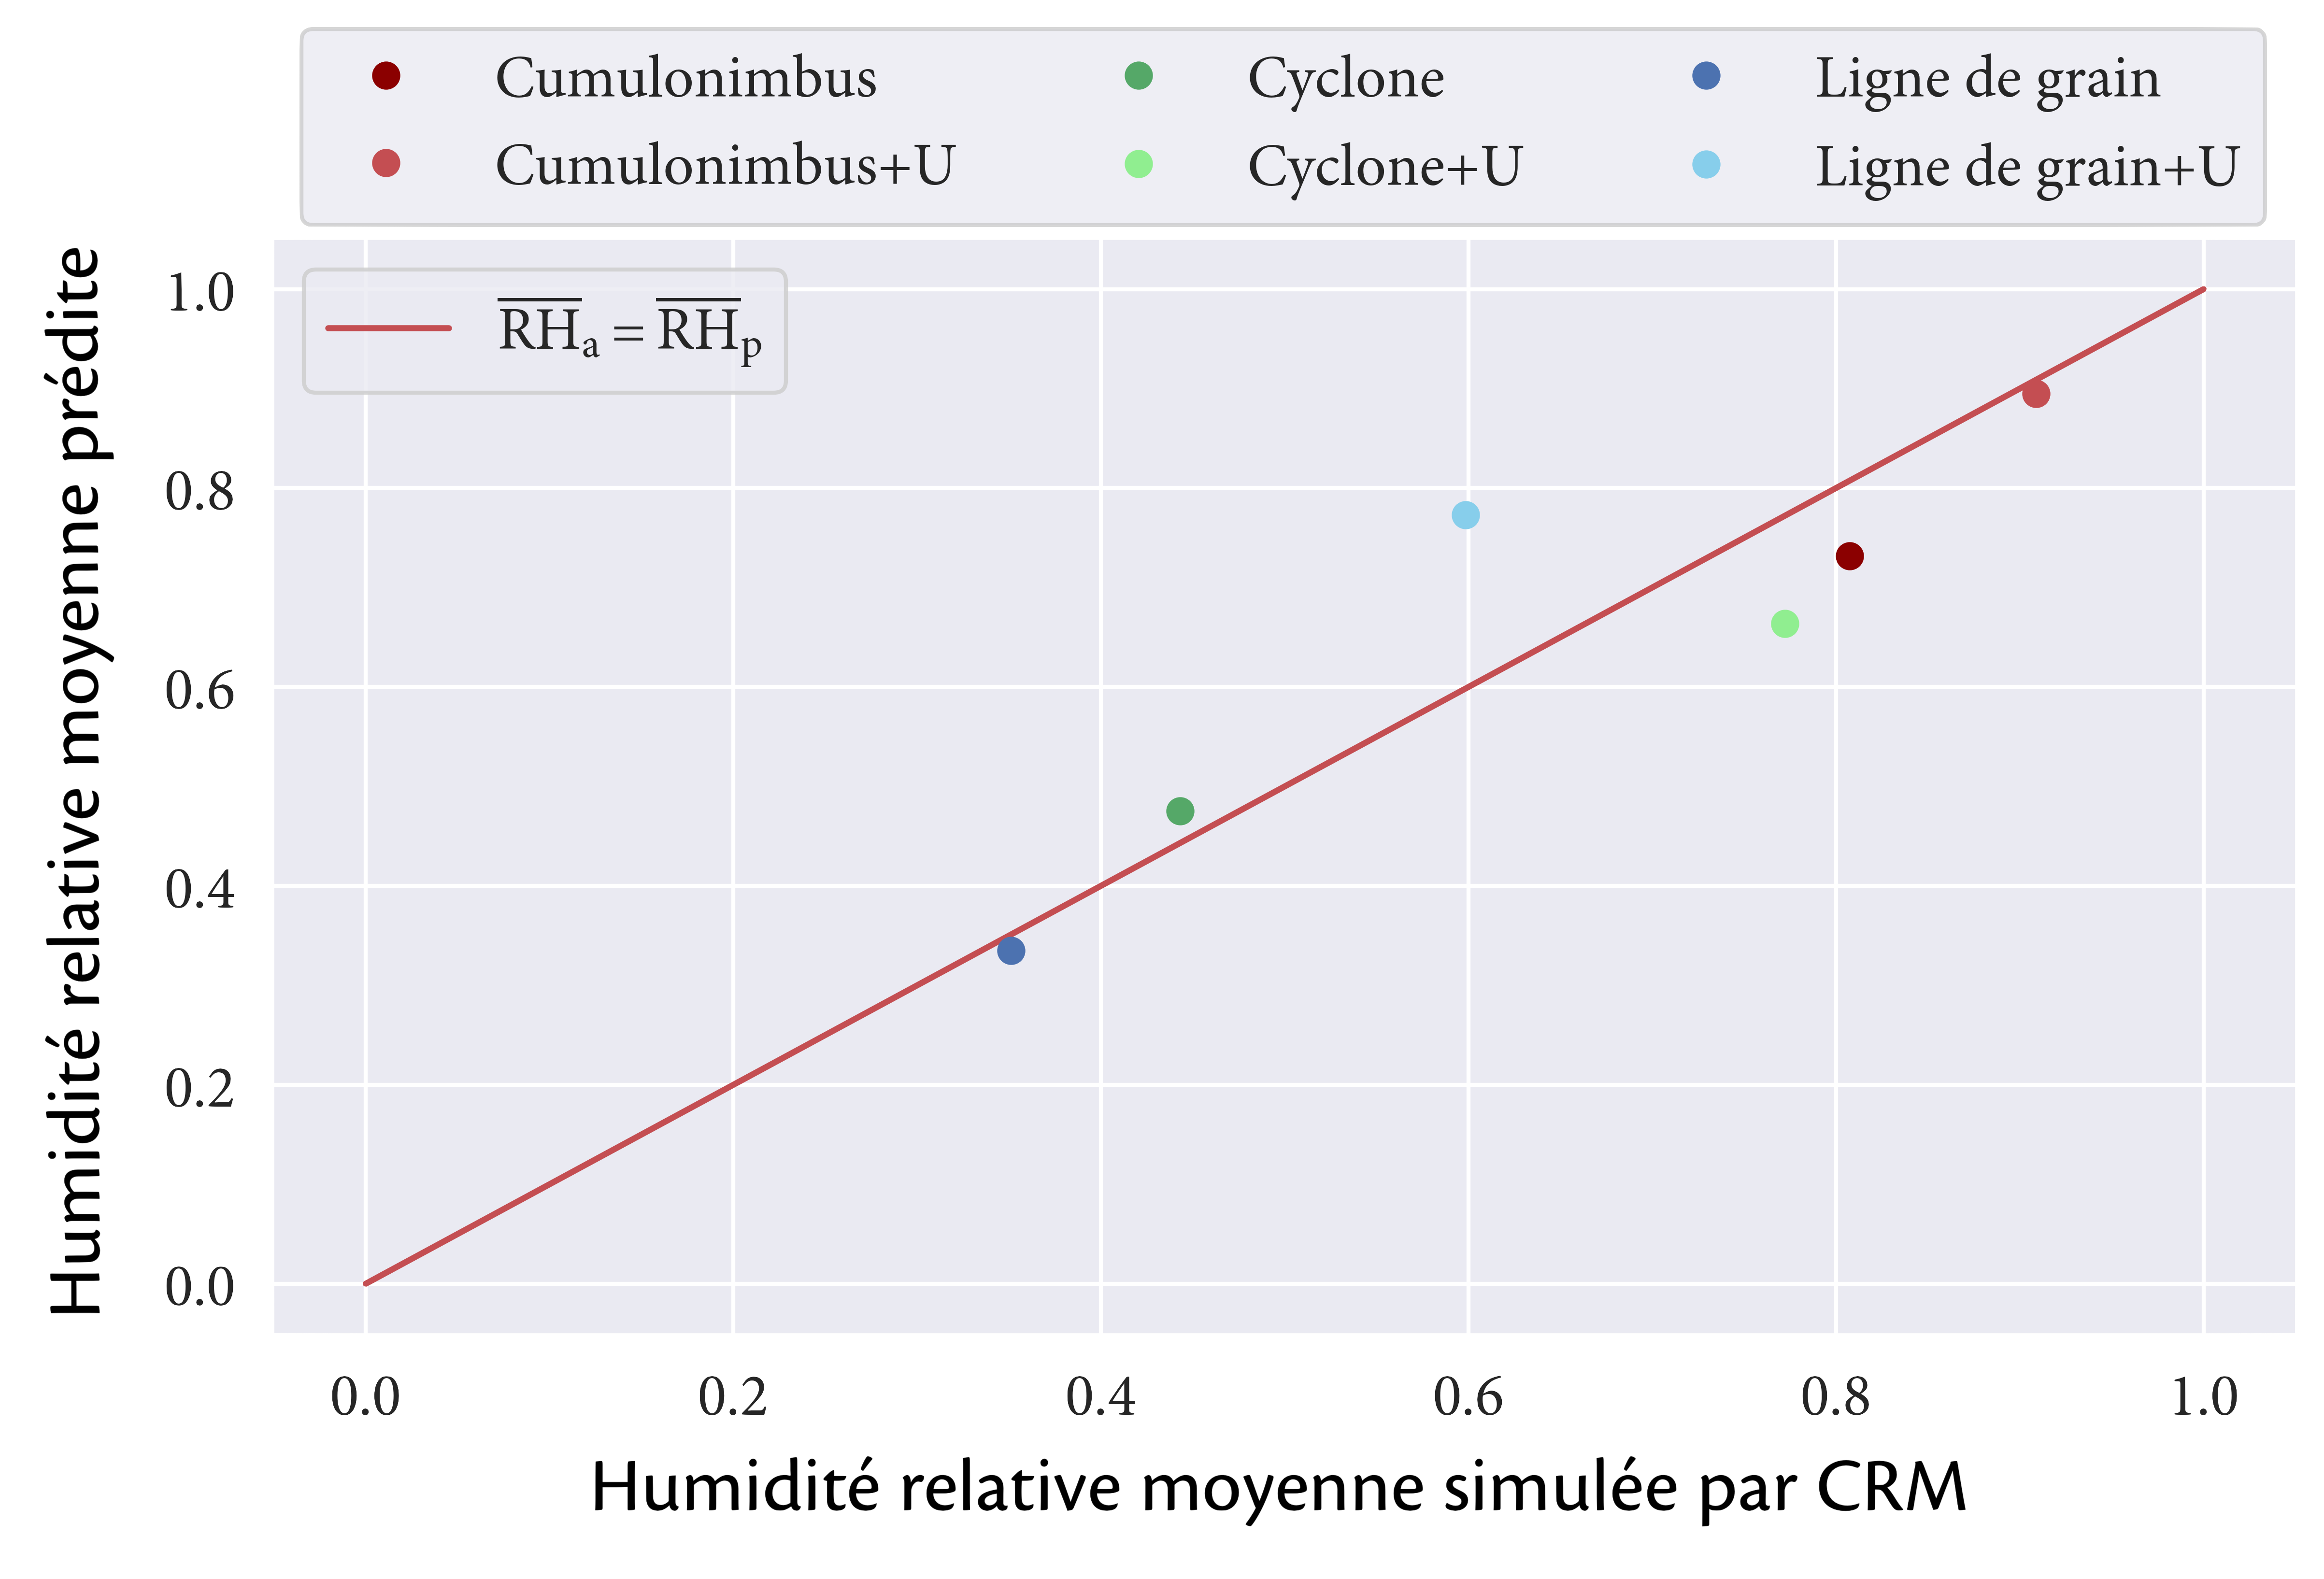
\includegraphics[width=7cm]{../Codes/Figs/meanRHpvsRHa.png} \hfill
    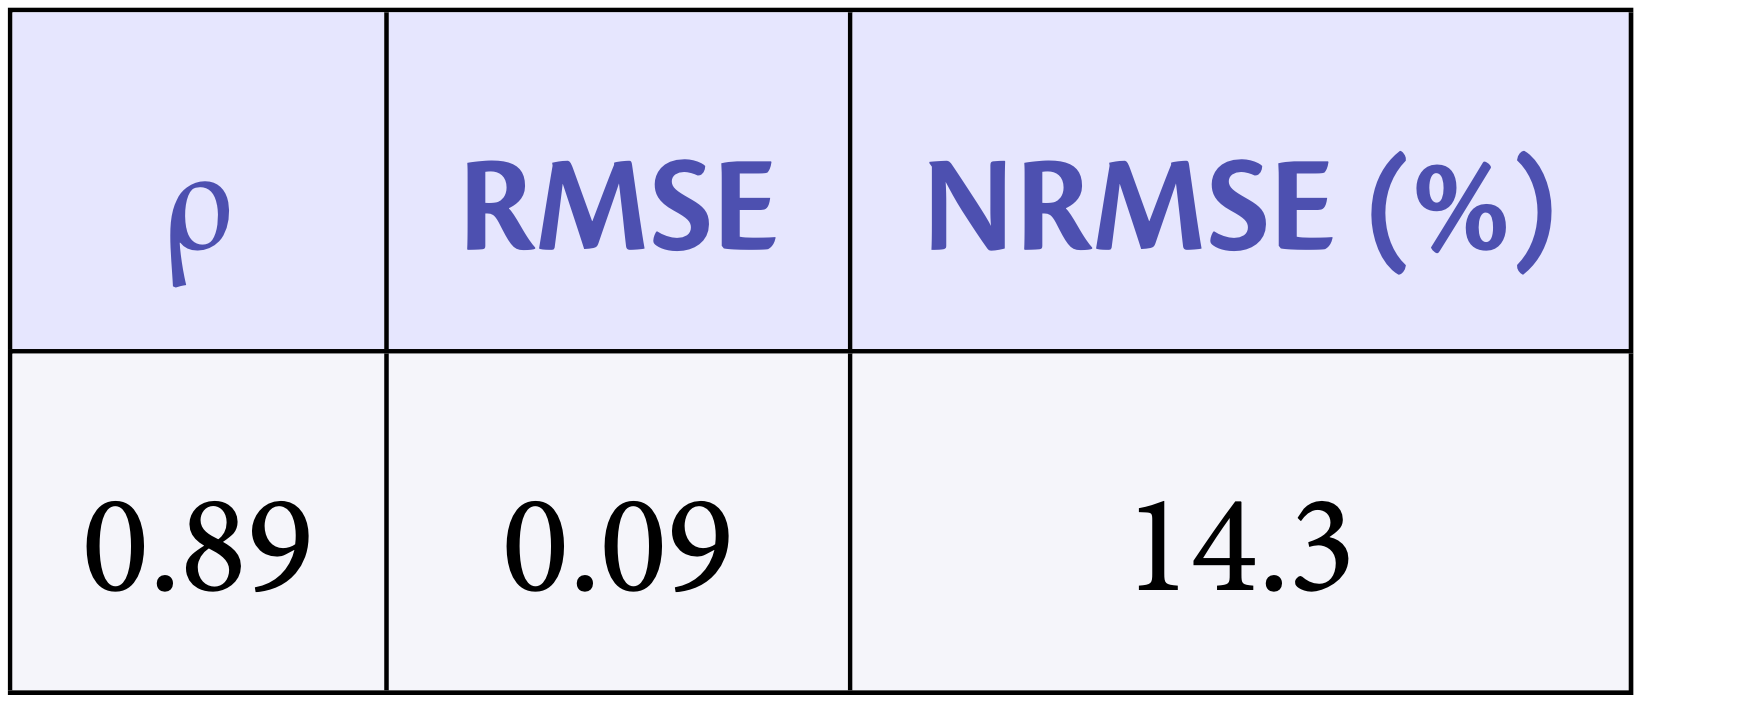
\includegraphics[width=4.5cm]{Figures/Table2.png}
\end{figure}
\vspace{0.1cm}
$\rightarrow \overline{RH}$ prédite par le modèle AC correspond à $\overline{RH}$ du CRM \\
$\rightarrow$ hypothèse valide: $\overline{RH}$ prédite à partir de la dynamique seulement.
}
\end{frame}

\begin{frame}{\secname}
\Wider{
On utilise la simplicité du modèle AC pour décortiquer les différences d'humidités entre simulations désorganisées et organisées 
\begin{figure}[hbtp]
    \centering
    \includegraphics[width=11.2cm]{../Codes/Figs/OrgComps.png}
\end{figure}
}
\end{frame}

\section*{Conclusion}
\begin{frame}{\secname}
\Wider{
\begin{block}{\vspace{-2.5ex}}
    L'assèchement moyen de la troposphère avec l'organisation est prédit avec un modèle sans considérations microphysiques
\end{block}
\pause
\vspace{-0.5cm}
\begin{block}{\vspace{-2.5ex}}
    Le changement d'intermittence des nuages est le principal facteur d'assèchement de la troposphère
\end{block}
\centering
\includegraphics[width=8cm]{Figures/SchémaBilan.png}
}
\end{frame}

{\usebackgroundtemplate{\tikz\node[opacity=0.2]{\includegraphics[width=21cm]{/Users/felixlangot/Google Drive (felixlangot@gmail.com)/UVSQ/Gestion de Projet/Poster/wallpaper2you_568686.jpg}};}
\begin{frame}
  \centering
  \Large 
  \textcolor{black}{Merci pour votre attention!}
\end{frame}
}

\section*{Influence du pas de temps}

\begin{frame}{\secname}

    \begin{figure}[hbtp]
        \centering
        \includegraphics[width=10cm]{../Codes/Figs2/RHps.png}
    \end{figure}
    
\end{frame}

\begin{frame}{\secname}
    \begin{figure}[hbtp]
        \centering
        \includegraphics[width=11.5cm]{../Codes/Figs2/meanRHvsDt.png}
    \end{figure}
\end{frame}

% \section*{Perspectives}
% \begin{frame}{\secname}
% \Wider{
% \begin{itemize}
%     \item Convergence: $\rightarrow$ Réduction du pas de temps \\
% ~~~~~~~~~~~~~~~~~~~~~~ $\rightarrow$ Cas de convection + organisée
%     \item $RH$ sous-estimée: Pourquoi? Comment corriger? \\
%         On ne considère pas:
%     \begin{itemize}
%         \item Les mouvements horizontaux $\rightarrow$ diminution de la probabilité de rencontrer un nuage
%         \item L'évaporation des hydrométéores \\ 
%     \end{itemize}
% ~~~~ + Trajectoire discrétisée \\
%     $\rightarrow$ Considérer une frange d'humidification autour des nuages ? \\
%     \begin{itemize}
%         \item Probabilité fixe sur une certaine distance/exponentielle décroissante avec la distance au nuage?
%     \end{itemize}
%     \item Prédire la RH avec quelques paramètres d'agrégation?
% \end{itemize} 
% }
% \end{frame}
% \begin{frame}[allowframebreaks]{Bibliographie}
%     \printbibliography
% \end{frame}

% \begin{frame}{Commentaires}
%     \begin{itemize}
%         \item Figure CRM: Ascendance couvre tout le domaine
%         \item 5km = exemple. Le but c'est de regarder la moyenne trop. dans son ensemble (Trop libre)
%         \item L'advec-cond. marche dans la trop. libre 
%         \item Enclume horizontale
%         \item prob. d'humidification $\rightarrow$ de saturation
%         \item Seuil nuage: article original
%     \end{itemize}
% \end{frame}

% \begin{frame}
%     \begin{itemize}
%         \item z$_{clouds}$ pour les autres simulations 
%         \item Ne pas dire que ça ne marche pas. On s'attend à ce que ça ne marche pas. On vérifie que l'intermittence des nuages est importante.
%         \item Résultat intéressant car simple a comprendre.
%     \end{itemize}
% \end{frame}

\end{document}
